\section{Instruction memory}
\subsubsection{Overview}
To execute any operation, the first step involves fetching the instruction from memory. To prepare for the next instruction, we increment the program counter so it points to the subsequent instruction's address, typically advancing by 4 bytes. This setup forms a datapath that handles instruction fetching and program counter incrementation for sequential instruction execution.

\subsubsection{Design Requirements}
\begin{itemize}
    \item \textbf{Memory Size:} 128 bytes (32 32-bit instructions). 
    \item \textbf{Data Bus Widths:}
    \begin{itemize}
    \item \textbf{Program Counter (PC):} 64 bits
    \item \textbf{Flash Instruction Input (flashInstruction):} 8 bits
    \item \textbf{Instruction Output: } 32 bits
    \item \textbf{Program Counter Bypass Output (pcBypass): } 64 bits 
    %\begin{tikzpicture}[baseline={([yshift=-.8ex]current bounding box.center)}]
   
    \end{itemize}
    \begin{figure}[H]
    \centering
    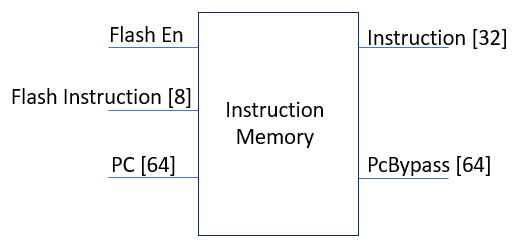
\includegraphics[width=0.5
    \linewidth]{Image/Instruction_Memory.png}
    \caption{Instruction Memory}
    \label{fig:enter-label}
\end{figure}
\end{itemize}
\subsubsection{Implementation Approach}
The implementation approach for the instructionMemory module involves the following key components and strategies:
\begin{itemize}
    \item \textbf{Memory Array:} A 128-byte internal memory array (instructionMem) is used to store the instructions. Each byte in this array represents a portion of the stored instructions.
    \item \textbf{Conditional Operation:} The module uses conditional logic to switch between flash programming mode and instruction fetch mode based on the state of the flashEn signal. This is achieved through a combination of always blocks and conditional assignments.
    \item \textbf{Byte Concatenation:} During instruction fetch mode, the module concatenates four consecutive bytes from the memory array to form a 32-bit instruction. This ensures that the CPU can retrieve complete instructions for execution.
    \item \textbf{Address Management:} The pcBypass output provides an alternative address for the program counter when flash programming is active. This helps in managing the program flow during memory updates.

\end{itemize}

\subsubsection{Detailed Functioning}
\begin{itemize}
    \item \textbf{Program Counter Bypass (pcBypass):} Set to 64'dX when flashEn is high, indicating an undefined state and halting normal PC operation.
    \item \textbf{Conditional Operation:} Writes flashInstruction[7:0] into instructionMem at the PC-specified address.Sets Instruction[31:0] to 32'dX during programming.
    \item \textbf{Instruction Memory Read (flashEn low):} Populates instruction with a 32-bit instruction fetched from instructionMem.\\
    Constructs the fetched instruction by concatenating four 8-bit segments from instructionMem.

\end{itemize}
